\chapter{Thermometry of an ultracold ideal fermi gas}
\label{ch:idealfermigas}
The purpose of the camera is to measure scientifically important data from dense atomic clouds consisting of Lithium and Caesium.
The improvement of the resolution in the whole imaging setup now allows to explore new attributes that could not be measured before and as an example, ultracold ideal Fermi Gases were chosen. They are apparent at very low temperatures, where only few atoms due to evaporative cooling are present. Their density distribution differs slightly from a gaussian form and from that, one can extract temperatures and atom numbers.

In order to image the atoms, a technique called absorption imaging is used which is explained in the next section, before the introduction to ideal Fermi Gases.

\section{Absorption imaging}
In order to find microscopic attributes of atoms, or systems of atoms, it is necessary to look at the atoms themselves. This is commonly accomplished using either fluorescence or absorption imaging\cite{Murmann2011}. In both cases, a laser beam is pointed at an atomic cloud, that is cooled and confined in a trap. In fluorescence imaging, the scattered light is collected, typically in a direction that is different than the illuminating beam.
The intensity from the light through this method is not very high, since it is radiated in all directions. Therefore, long exposure times are required during which atoms can move and the information about the initial density and energy distribution is lost. Nevertheless, it is useful for single- and few-atom detection.

In contrast, in absorption imaging\cite{helmrich2013}, the transmitted intensity of the imaging beam is recorded. Without atoms, one would see a beam profile of the laser beam. With atoms, a shadow is visible due to the atoms "blocking" the light. This is accomplished, by correctly tuning the laser to a resonance frequency of the atoms, which enables them to absorb the light, exciting them to a higher state. Through spontaneous emission, the atoms will decay, making it possible to excite them once again. This method works well, when the "signal" from the absorbed light is significantly larger compared to the noise sources.

There are a set of optical elements in the imaging path, like lenses to collimate the image and refocus it, or mirrors to guide the light into the camera. Since the surfaces will most likely introduce errors into the imaging, for example from impurities or dust, only the absorption image will not suffice to gain reliable data. This is compensated by taking a total of three pictures, in order to extract only the relevant information from the image.

This can be understood when looking at the light intensity $I_{CCD}$ reaching the camera. The atom cloud has an optical density $OD$, therefore the intensity can be written as\cite{Murmann2011}
\begin{equation}
I_{CCD} = I_0 e^{-OD} + I_{back},
\end{equation}
where it decreases from the incident laser intensity $I_0$ due to light scattering by atoms. The intensity $I_{back}$ describes the background signal, that is found when the CCD is not being illuminated by a laser such as readout noise, dark noise or stray photon light. All the interesting attributes of atoms are found by looking at the optical density, therefore in order to extract that, a background frame is subtracted from the absorption image and the laser profile divided, leaving
\begin{equation}
\frac{I_{CCD} - I_{back}}{I_0} = e^{-OD}.
\end{equation}
The laser intensity $I_0$ is measured in a separate frame, containing the laser intensiy $I_0' = I_0 + I_{back}$ and also the background $I_{back}$. Finally, the equation yields
\begin{equation}
\frac{I_{CCD} - I_{back}}{I_0' - I_{back}} = e^{-OD}.
\end{equation}

From the resulting optical density, one can now conclude, for example, atom density distributions, atom numbers or excitation rates.

\section{Density distributions of ideal Fermi gases}
\label{sec:densdistrfermi}

Ideal Fermi gases offer a new aggregate, that is complementary to Bose-Einstein condensate. They are found on the Bardeen-Cooper-Schrieffer side of the Feshbach resonances as a polarized species with only one spin component. At very cold temperatures, they start to differ from a gaussian distribution which is further investigated in this chapter.

The distribution of the atoms depends on the fraction of their temperature to the Fermi temperature\cite{Ketterle2008} $T_F$. For $T/T_F \gg 1$, the atoms will follow a gaussian distribution, which can be identified using the gaussian radius:
\begin{equation}
\sigma _i = \sqrt{\frac{2k_BT}{mw_i^2}},
\end{equation}
with the mass of Lithium $m$ and the trapping frequency $w_i$ in the direction of the radius. Due to the alignment of the dipole trap, the cloud will not have a spherical shape and will therefore have different radii.

In the degenerate regime however, for $T/TF \ll 1$, the radius is described by the Fermi radius
\begin{equation}
R_{Fi} = \sqrt{\frac{2E_F}{mw_i^2}},
\end{equation}
using the Fermi energy $E_F$, due to the fermions filling up the eigenstates of the potential.

It is therefore suggested\cite{Ketterle2008} to use a unified radius, as the temperatures are not known a priori:
\begin{equation}
R_i^2 = \frac{2k_BT}{mw_i^2}f( e^{\frac{\mu}{k_BT}}).
\end{equation}
The interpolation function $f(x)$ is hereby:
\begin{equation}
f(x) = \frac{Li_1(-x)}{Li_0(-x)}
\end{equation}
where $Li_n$ is polylogarithm and can be defined as
\begin{equation}
Li_s(z) = \sum_{k=1}^{\infty} \frac{z^k}{k^s}.
\end{equation}

In our case, we integrate over all but one axes, and therefore find the fitting function for the atom numbers:
\begin{equation}
\label{eq:n1d}
n_{1D}(x) = n_{1D,0}\frac{Li_{5/2}\left( \pm \mathrm{exp}\left[ q-\frac{x^2}{R_x^2}f(e^q)\right] \right)}{Li_{5/2}(\pm e^q)}.
\end{equation}
The derivation can be found in \cite{Ketterle2008}. The parameter $q=\frac{\mu}{k_BT}$ can be extracted, which contains information about the chemical potential $\mu$ and the temperature $T$.

This parameter can then be used to calculate the degeneracy parameter:
\begin{equation}
\label{eq:tovertf}
\frac{T}{T_F} = \left[ -6 Li_3(-e^q) \right]^{-1/3}.
\end{equation}

To compensate for the finite resolution of the chip on the camera, the cloud can be imaged after a short time of flight $t$. The temperature can then be calculated from the dynamics as
\begin{equation}
\label{eq:temp}
k_BT = \frac{1}{2} mw_i^2 \frac{R_i^2}{1+w_i^2t^2}\frac{1}{f(e^q)}.
\end{equation}


	
\section{Finding properties of the Fermi gas}

As seen before, from an ideal Fermi gas, one can deduce the temperature and Fermi temperature of a gas.
In order to implement ideal Fermi gases, Lithium was prepared in an optical dipole trap. The power was ramped down several times at the Feshbach resonance $B=\SI{896}{\gauss}$, until only a fraction of the atoms remained. The spin-down atoms received a short laser pulse, so that the cloud only consisted of spin-up $^6$Li.

\pltCustom{
	\begin{center}
		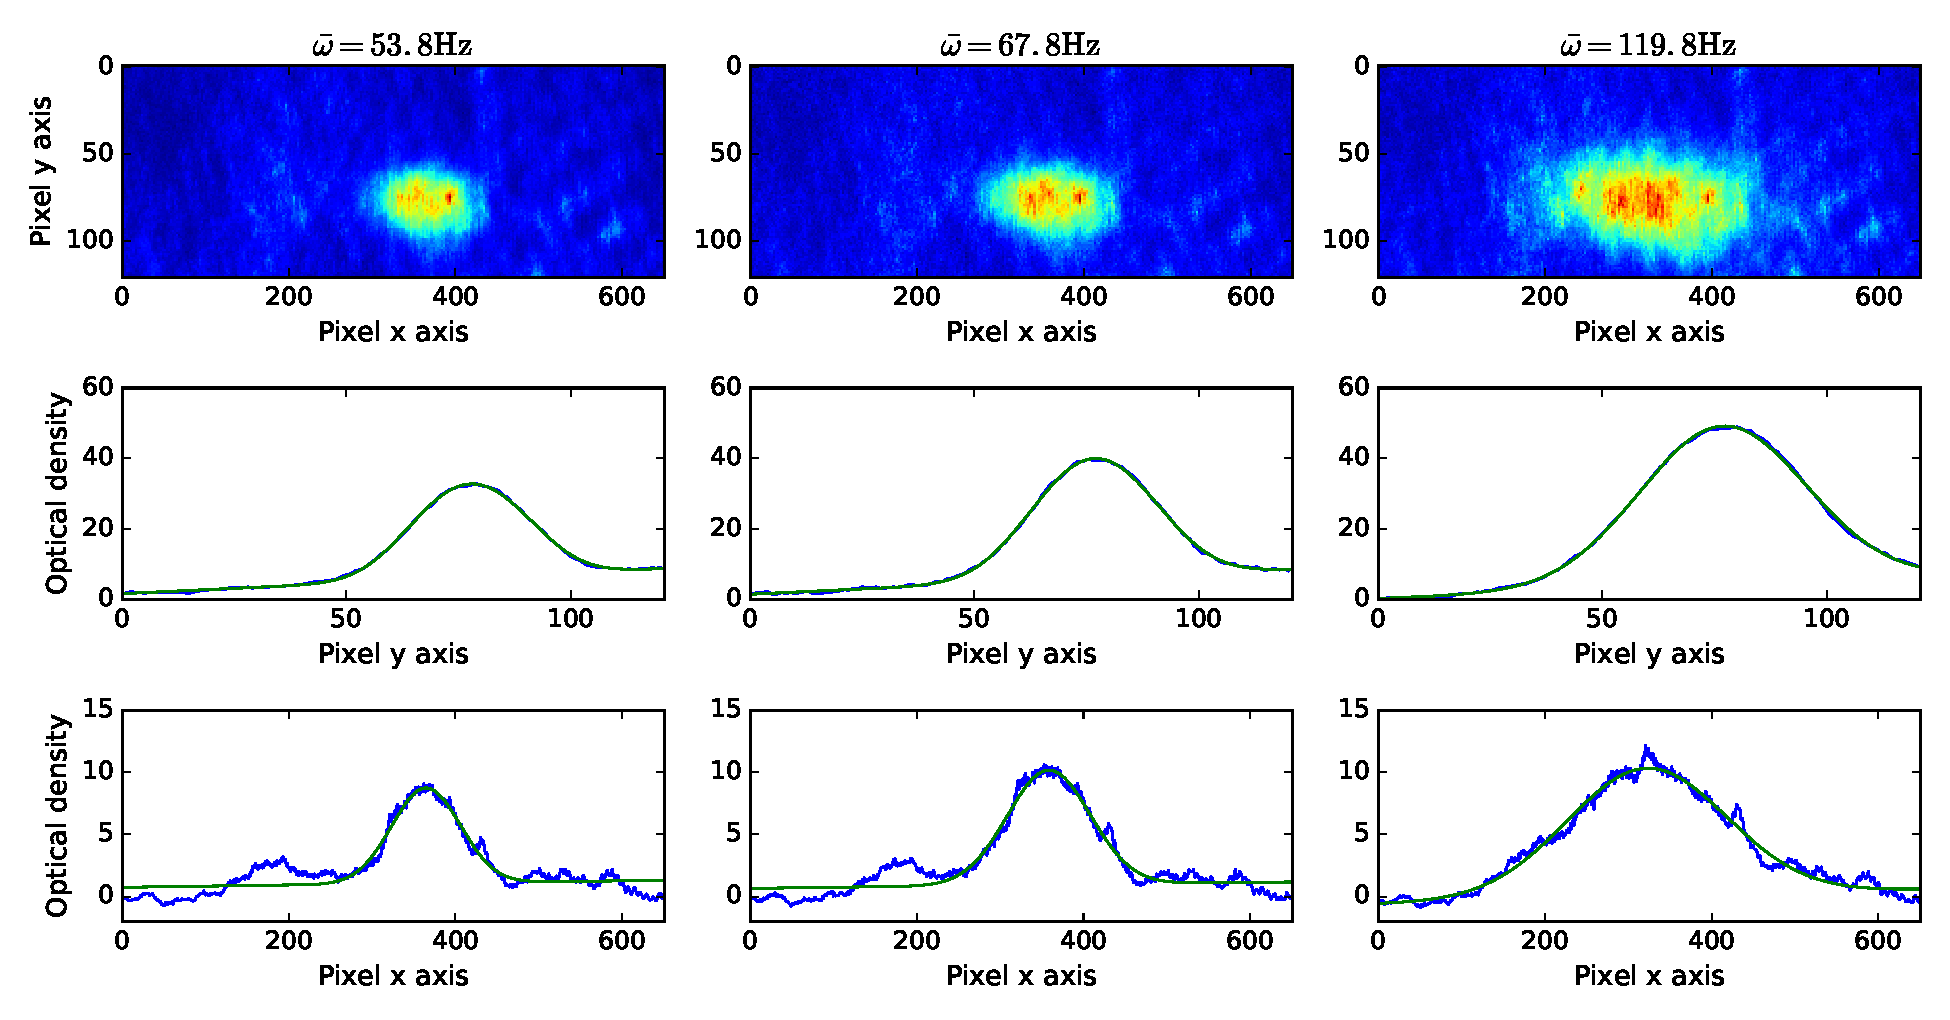
\includegraphics[width=1\textwidth]{drafts/fermi_fit.pdf}
	\end{center}
	\begin{textblock}{2}(0.75,-4.7)
		\textbf{a.}
	\end{textblock}
	\begin{textblock}{2}(4.55,-4.7)
		\textbf{b.}
	\end{textblock}
	\begin{textblock}{2}(8.35,-4.7)
		\textbf{c.}
	\end{textblock}
}{fermi_fit}{Fitting the fermi distribution to an ideal Fermi gas}{In order to find the physical properties of a fermionic cloud, they were imaged at three different trap depths which correspond to the $\bar{\omega} = (\omega_x \omega_y \omega_z)^{1/3}$, where $w_i$ is the trap frequency in the corresponding axis. As of the writing of this thesis, the imaging system was not yet well aligned in the x-Direction, therefore the data does not represent the theory well. The results of the fits are given in Table \ref{tab:fermi_fit}.}

The measurement was executed for three different powers of the laser beam. The atoms were imaged after a short time of flight of \SI{1}{\milli\second}. In order to fit the function \refEq{n1d}, the absorption image yielding the optical density as seen in \refFig{fermi_fit} was integrated over one axis, giving a one dimensional distribution for the atoms.

As the imaging is not properly optimized at this point, the distribution in the horizontal (x-axis) direction does not represent the theory well, even after averaging over several acquisitions. This problem could not be resolved due to timing constrictions, therefore the fit parameters were extracted solely from the vertical direction.

On the vertical axis, a common systematic error was a small peak for high values, which did not correspond to the atoms and is probably due to the lenses, which are not properly aligned. This was excluded from the fit. Due to the alignment in the x-Direction, the measurement could not be included, as the fragments disturbed the data too much.
\begin{table}
	\begin{center}
		\begin{tabular}{M{1cm}!M{4cm}|M{4cm}|M{4cm}N}
			& $\bar{\omega}=\SI{53.8}{\hertz}$ & $\bar{\omega}=\SI{67.8}{\hertz}$ & $\bar{\omega}=\SI{119.8}{\hertz}$ & \\[7pt]
			\thickhline
			$n_{1D}$ & $25.6\pm0.1$ & $34.07\pm0.13$ & $44.98\pm0.24$ & \\ [7pt]
			\hline
			$q$ & $1.87\pm0.35$ & $1.08\pm0.34$ & $-2.0\pm1.85$ & \\[7pt]
			\hline
			$R_y$ & $23.9\pm0.72$ & $23.80\pm0.75$ & $26.79\pm1.06$ & \\[7pt]
			\hline
			$T$ & $(5.92\pm0.55)*10^{-8}$ & $(7.43\pm0.14)*10^{-7}$ & $(1.23\pm0.25)*10^{-6}$ & \\[7pt]
			\hline
			$T/T_F$ & $0.34$ & $0.42$ & $1.01$ & \\[7pt]
		\end{tabular}
	\end{center}
	\setCaption{Fit parameters for various trap depths}{The Fermions were fitted using \refEq{n1d}, where the parameter $n_{1D}$ describes the amplitude of the peak. $q$ is a shape parameter, which is negative if the cloud is thermal or positive if the cloud is degenerate. $R_y$ is then the clouds radius similar as the radius can be described in a gaussian distribution which is in units of pixels and can be calculated in natural units using the pixel size (\SI{13}{\micro\meter}) and the magnification ($7.5$).}
	\label{tab:fermi_fit}
\end{table}

In order to properly fit \refEq{n1d}, a linear function had to be added, as there was a constrant gradient on the chip, most likely due to the readout of the image. From the fit parameters in Table \ref{tab:fermi_fit}, it was possible to calculate the temperature and the degeneracy parameter from \ref{eq:temp} and \ref{eq:tovertf} respectively. From the results of $T/T_F$ it can be seen, that the gas is becoming more degenerate, as the trapping frequencies become lower. Additionally, the temperature of the gas is becoming cooler, as more atoms leave the trap, which is expected from evaporative cooling as well.

This experiment already shows the operation of the camera as a scientific instrument. As predicted from theory \cite{Ketterle2008}, the gas follows a Fermi distribution as the cloud becomes colder.